\documentclass[11pt,preprint, authoryear]{elsarticle}

\usepackage{lmodern}
%%%% My spacing
\usepackage{setspace}
\setstretch{1.2}
\DeclareMathSizes{12}{14}{10}{10}

% Wrap around which gives all figures included the [H] command, or places it "here". This can be tedious to code in Rmarkdown.
\usepackage{float}
\let\origfigure\figure
\let\endorigfigure\endfigure
\renewenvironment{figure}[1][2] {
    \expandafter\origfigure\expandafter[H]
} {
    \endorigfigure
}

\let\origtable\table
\let\endorigtable\endtable
\renewenvironment{table}[1][2] {
    \expandafter\origtable\expandafter[H]
} {
    \endorigtable
}


\usepackage{ifxetex,ifluatex}
\usepackage{fixltx2e} % provides \textsubscript
\ifnum 0\ifxetex 1\fi\ifluatex 1\fi=0 % if pdftex
  \usepackage[T1]{fontenc}
  \usepackage[utf8]{inputenc}
\else % if luatex or xelatex
  \ifxetex
    \usepackage{mathspec}
    \usepackage{xltxtra,xunicode}
  \else
    \usepackage{fontspec}
  \fi
  \defaultfontfeatures{Mapping=tex-text,Scale=MatchLowercase}
  \newcommand{\euro}{€}
\fi

\usepackage{amssymb, amsmath, amsthm, amsfonts}

\def\bibsection{\section*{References}} %%% Make "References" appear before bibliography


\usepackage[round]{natbib}

\usepackage{longtable}
\usepackage[margin=2.3cm,bottom=2cm,top=2.5cm, includefoot]{geometry}
\usepackage{fancyhdr}
\usepackage[bottom, hang, flushmargin]{footmisc}
\usepackage{graphicx}
\numberwithin{equation}{section}
\numberwithin{figure}{section}
\numberwithin{table}{section}
\setlength{\parindent}{0cm}
\setlength{\parskip}{1.3ex plus 0.5ex minus 0.3ex}
\usepackage{textcomp}
\renewcommand{\headrulewidth}{0pt}

\usepackage{array}
\newcolumntype{x}[1]{>{\centering\arraybackslash\hspace{0pt}}p{#1}}

%%%%  Remove the "preprint submitted to" part. Don't worry about this either, it just looks better without it:
\makeatletter
\def\ps@pprintTitle{%
  \let\@oddhead\@empty
  \let\@evenhead\@empty
  \let\@oddfoot\@empty
  \let\@evenfoot\@oddfoot
}
\makeatother

 \def\tightlist{} % This allows for subbullets!

\usepackage{hyperref}
\hypersetup{breaklinks=true,
            bookmarks=true,
            colorlinks=true,
            citecolor=blue,
            urlcolor=blue,
            linkcolor=blue,
            pdfborder={0 0 0}}


% The following packages allow huxtable to work:
\usepackage{siunitx}
\usepackage{multirow}
\usepackage{hhline}
\usepackage{calc}
\usepackage{tabularx}
\usepackage{booktabs}
\usepackage{caption}


\newenvironment{columns}[1][]{}{}

\newenvironment{column}[1]{\begin{minipage}{#1}\ignorespaces}{%
\end{minipage}
\ifhmode\unskip\fi
\aftergroup\useignorespacesandallpars}

\def\useignorespacesandallpars#1\ignorespaces\fi{%
#1\fi\ignorespacesandallpars}

\makeatletter
\def\ignorespacesandallpars{%
  \@ifnextchar\par
    {\expandafter\ignorespacesandallpars\@gobble}%
    {}%
}
\makeatother

\newenvironment{CSLReferences}[2]{%
}

\urlstyle{same}  % don't use monospace font for urls
\setlength{\parindent}{0pt}
\setlength{\parskip}{6pt plus 2pt minus 1pt}
\setlength{\emergencystretch}{3em}  % prevent overfull lines
\setcounter{secnumdepth}{5}

%%% Use protect on footnotes to avoid problems with footnotes in titles
\let\rmarkdownfootnote\footnote%
\def\footnote{\protect\rmarkdownfootnote}
\IfFileExists{upquote.sty}{\usepackage{upquote}}{}

%%% Include extra packages specified by user

%%% Hard setting column skips for reports - this ensures greater consistency and control over the length settings in the document.
%% page layout
%% paragraphs
\setlength{\baselineskip}{12pt plus 0pt minus 0pt}
\setlength{\parskip}{12pt plus 0pt minus 0pt}
\setlength{\parindent}{0pt plus 0pt minus 0pt}
%% floats
\setlength{\floatsep}{12pt plus 0 pt minus 0pt}
\setlength{\textfloatsep}{20pt plus 0pt minus 0pt}
\setlength{\intextsep}{14pt plus 0pt minus 0pt}
\setlength{\dbltextfloatsep}{20pt plus 0pt minus 0pt}
\setlength{\dblfloatsep}{14pt plus 0pt minus 0pt}
%% maths
\setlength{\abovedisplayskip}{12pt plus 0pt minus 0pt}
\setlength{\belowdisplayskip}{12pt plus 0pt minus 0pt}
%% lists
\setlength{\topsep}{10pt plus 0pt minus 0pt}
\setlength{\partopsep}{3pt plus 0pt minus 0pt}
\setlength{\itemsep}{5pt plus 0pt minus 0pt}
\setlength{\labelsep}{8mm plus 0mm minus 0mm}
\setlength{\parsep}{\the\parskip}
\setlength{\listparindent}{\the\parindent}
%% verbatim
\setlength{\fboxsep}{5pt plus 0pt minus 0pt}



\begin{document}



\begin{frontmatter}  %

\title{Helpful insights for starting a streaming service}

% Set to FALSE if wanting to remove title (for submission)




\author[Add1]{Tessa Hubble}
\ead{21559953@sun.ac.za.com}





\address[Add1]{Stellenbosch University, South Africa}


\begin{abstract}
\small{
This report will offer some insight into which genres would be
adavnatageous to add to a streaming service among movies and series as
well as which actors signal popular films.
}
\end{abstract}

\vspace{1cm}





\vspace{0.5cm}

\end{frontmatter}

\setcounter{footnote}{0}



%________________________
% Header and Footers
%%%%%%%%%%%%%%%%%%%%%%%%%%%%%%%%%
\pagestyle{fancy}
\chead{}
\rhead{}
\lfoot{}
\rfoot{}
\lhead{}
%\rfoot{\footnotesize Page \thepage } % "e.g. Page 2"
\cfoot{}

%\setlength\headheight{30pt}
%%%%%%%%%%%%%%%%%%%%%%%%%%%%%%%%%
%________________________

\headsep 35pt % So that header does not go over title




\hypertarget{introduction}{%
\section{\texorpdfstring{Introduction
\label{Introduction}}{Introduction }}\label{introduction}}

A streaming service has to carefully select titles that will draw users
to the platform. Series and movies genres therefore present an important
aspect of the service. Figure 1 and 2 show the frequency of genres among
series and movies with an imdb score of above 8. For the last 10 years,
drama as a genre has dominated the most popular series. The next most
frequent genre among the most popular series, is comedies. Documentaries
tend to come up in around 25 percent of popular series. In 2022, there
appears to be a spike in the popularity of the romance genre.

\begin{figure}[H]

{\centering \includegraphics{Question_4_files/figure-latex/Figure1-1} 

}

\caption{Frequency of genres among popular series  \label{Figure1}}\label{fig:Figure1}
\end{figure}

Among popular movies, dramas continue to appear frequently.
Documentaries and comedies also perform consistently, although at lower
frequencies. Actions and animation movies tend to feature less and less
among popular movies over time.

\begin{figure}[H]

{\centering 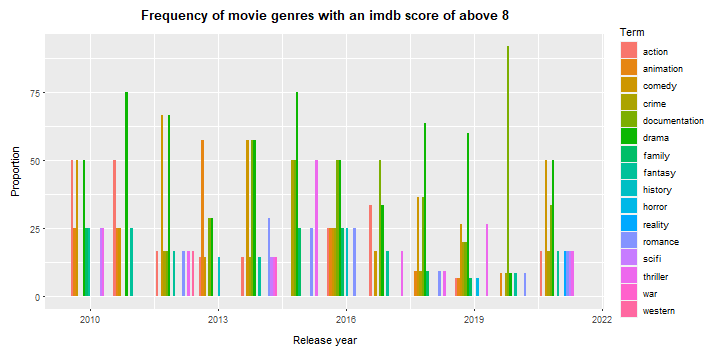
\includegraphics{Question_4_files/figure-latex/Figure2-1} 

}

\caption{Frequency of genres among popular movies \label{Figure2}}\label{fig:Figure2}
\end{figure}

The table below shows the most popular actors, their average imdb rating
and their most popular movie or series performance. It becomes clear
that including series in a streaming performance is of the utmost
importance. More so, including very popular series within the last two
decades should bring in users to the platform. Series and movies with
the following actors are likely to incentivise users to join.

\begin{verbatim}
## \begin{table}[ht]
## \centering
## \begin{tabular}{rlrllr}
##   \hline
##  & Name & Average imdb score & Highest rated movie/series & Type & Release year \\ 
##   \hline
## 1 & Anna Gunn & 9.50 & Breaking Bad & SHOW & 2008.00 \\ 
##   2 & Betsy Brandt & 9.50 & Breaking Bad & SHOW & 2008.00 \\ 
##   3 & Cricket Leigh & 9.30 & Avatar: The Last Airbender & SHOW & 2005.00 \\ 
##   4 & Jessie Flower & 9.30 & Avatar: The Last Airbender & SHOW & 2005.00 \\ 
##   5 & Zach Tyler & 9.30 & Avatar: The Last Airbender & SHOW & 2005.00 \\ 
##   6 & He Kailang & 9.20 & Who Rules The World & SHOW & 2022.00 \\ 
##   7 & Kim Seol & 9.20 & Reply 1988 & SHOW & 2015.00 \\ 
##   8 & Lee Hye-ri & 9.20 & Reply 1988 & SHOW & 2015.00 \\ 
##   9 & Lee Ji-ah & 9.20 & My Mister & SHOW & 2018.00 \\ 
##   10 & Ryu Jun-yeol & 9.20 & Reply 1988 & SHOW & 2015.00 \\ 
##   11 & Son Sook & 9.20 & My Mister & SHOW & 2018.00 \\ 
##   12 & Zhang Feng Yi & 9.20 & Who Rules The World & SHOW & 2022.00 \\ 
##   13 & Jason Hehir & 9.10 & The Last Dance & SHOW & 2020.00 \\ 
##   14 & Michael Jordan & 9.10 & The Last Dance & SHOW & 2020.00 \\ 
##   15 & Phil Jackson & 9.10 & The Last Dance & SHOW & 2020.00 \\ 
##   16 & Scottie Pippen & 9.10 & The Last Dance & SHOW & 2020.00 \\ 
##   17 & Steve Kerr & 9.10 & The Last Dance & SHOW & 2020.00 \\ 
##   18 & Alastair Fothergill & 9.00 & David Attenborough: A Life on Our Planet & MOVIE & 2020.00 \\ 
##   19 & Ariel Staltari & 9.00 & Okupas & SHOW & 2000.00 \\ 
##   20 & Augusto Brítez & 9.00 & Okupas & SHOW & 2000.00 \\ 
##    \hline
## \end{tabular}
## \end{table}
\end{verbatim}

\bibliography{Tex/ref}





\end{document}
